\section{Modelling} \label{sec:modelling}

\subsection{Simplifications}

All robots share some common modelling simplifications. The robot is assumed to be walking on a flat, horizontal surface at a constant velocity. Wind forces and joint friction are neglected and thus no horizontal forces are applied. The former is justified as being almost equally applicable to all topologies since the torso likely represents a much larger source of drag than the legs. Kalouche found in his 3-DoF parallel-articulated topology that the combined friction force of all actuators and joints amounted to less than $1N$ at the foot, for a peak output foot force of $130N$; friction is relatively small and will likely not vary much by topology \cite{kalouche_design_2016}. 

As the mass of ANYdrives is not available, HEBI Robotics X8-16 series-elastic actuators were used instead since their peak torque is within 5\% of ANYdrive \cite{hebi_robotics_x-series_nodate}\cite{hutter_anymal_2016}. Although required peak actuator torque varies as a function of the dynamic model, these actuators present sufficient torque to perform the deliberate motions anticipated for the intended application. Actuator inertias were neglected. 

Finally, each linkage is assumed to be constructed of Aluminium 6061 as a relatively lightweight and inexpensive material. Each link is composed of 6061 tube with an outer diameter of $0.044m$ and inner diameter of $0.0408m$; these were found to be sufficient for a $90kg$ five-legged robot \cite{arsenault_waterfront_2019}. While more dense than carbon fibre or fibreglass as employed on other quadrupeds, this is an economical material choice. The mass of each linkage is split evenly between its proximal and distal tips, alongside any actuator located at either joint joint.

%%%%%%%%%%%%%%%%%%%%%%%%%%%%%%%%%%%%%%%%%%%%%%%%%%%%%%%%%%%
%  3-DoF series-articulated
%%%%%%%%%%%%%%%%%%%%%%%%%%%%%%%%%%%%%%%%%%%%%%%%%%%%%%%%%%%
\subsection{3-DoF Series-Articulated}

\subsubsection{Forward and Inverse Kinematics}

This topology, found on MIT Cheetah 3, Mini Cheetah and ANYmal amongst others, will act as a reference leg design. The following procedure is derived from Spong and Wieber \cite{spong_robot_2020}\cite{wieber_modeling_2016}\cite{wieber_holonomy_2006}. First, the general homogenous transformation matrix from frame $i-1$ to $i$ \cite{spong_robot_2020}.

\begin{equation}
    T_{i-1}^{i} = \begin{bmatrix}
        \cos\theta_n & -\sin\theta_n\cos\alpha_n & \sin\theta_n\sin\alpha_n  & r_n\cos\theta_n \\
        \sin\theta_n & \cos\theta_n\cos\alpha_n  & -\cos\theta_n\sin\alpha_n & r_n\sin\theta_n \\
        0            & \sin\alpha_n              & \cos\alpha_n              & d_n \\
        0            & 0                         & 0                         & 1
    \end{bmatrix}
\end{equation}

\begin{figure}
    \centering
    \includegraphics[width=0.5\textwidth]{images/5/5_3dof-series-articulated-dh-parameters.png}
    \caption{Denavit-Hartenburg Parameters for 3-DoF series articulated leg topology}
    \label{fig:series-articulated-dh-params}
\end{figure}

The homogeneous transformation matrix from the hip to foot is given by

\begin{equation}
    T_0^4 = T_0^1 T_1^2 T_2^3 T_3^4= \left[\begin{matrix}- s_{1}  c_{34}  & s_{1}  s_{34}  & c_{1}  & \ell_{1} c_{1}  - \ell_{3} s_{1}  c_{3}  - \ell_{4} s_{1}  c_{34} \\c_{1}  c_{34}  & - s_{34}  c_{1}  & s_{1}  & \ell_{1} s_{1}  + \ell_{3} c_{1}  c_{3}  + \ell_{4} c_{1}  c_{34} \\s_{34}  & c_{34}  & 0 & \ell_{3} s_{3}  + \ell_{4} s_{34} \\0 & 0 & 0 & 1\end{matrix}\right]
\end{equation}

%While $\theta_1$ is present in the transformation matrix as a variable, for this thesis it shall be held as constant at $270^{\circ}$, with link $\ell_1$ parallel to the $y_0$ axis and as shown in Figure \ref{fig:series-articulated-dh-params}.

The forward kinematics are represented by the top three elements of the final row.

\begin{align}
    x_4 &= (T_0^4)_{0,3}
    \\
    y_4 &= (T_0^4)_{1,3}
    \\
    z_4 &= (T_0^4)_{2,3}
\end{align}

The inverse kinematics were derived using the procedure outlined in Spong for a robotic arm with shoulder \cite{spong_robot_2020}. The resulting joint angle equations are given by

\begin{align}
    \theta_1 &= \text{atan2}\big( \frac{y_4}{x_4}\big) - \text{atan2}\big(\frac{\sqrt{x_4^2 + y_4^2 - \ell_1^2}}{\ell_1} \big)
    \\
    \theta_2 &= \frac{\pi}{2}
    \\
    \theta_3 &= \text{atan2}\big( \frac{z_4}{\sqrt{x_4^2 + y_4^2 - \ell_1^2}} \big) - \text{atan2}\big( \frac{\ell_4\sin\theta_4}{\ell_3 + \ell_4\cos\theta_4} \big)
    \\
    \theta_4 &= \text{atan2}\big( \pm\frac{\sqrt{1-D^2}}{D} \big)
    \\
    D &= \frac{x_4^2 + y_4^2 + z_4^2 - \ell_1^2 - \ell_3^2 - \ell_4^2}{2\ell_3\ell_4}
\end{align}

\subsubsection{Jacobian}

The linear Jacobian represents the relationship between the linear joint velocities of a given joint in the base frame ($i=0$) and the joint velocities ($\dot{\theta_i}$).

\begin{equation} \label{eq:Jacobian-relation}
    v = J_v\dot{\theta}
\end{equation}

All terms of the Jacobian matrix can be found using the following relationship

\begin{equation} \label{eq:Jacobian-expression}
    J_{v_{jk}} = \frac{\partial p_j}{\partial q_k}
\end{equation}

where $p = [x y z]$ is the joint position as a function of the joint angles (the forward kinematics), $j$ the $j$-th joint coordinate (either $x$, $y$, or $z$), $q = [\theta_1 \theta_2 \theta_3]$ is the generalized coordinates, and $k$ is the $k$-th generalized coordinate. The resulting linear Jacobian for the foot is given by

\begin{equation}
    J_v = \left[\begin{matrix}- \ell_{1} s_{1} - \ell_{3} c_{1} c_{3} - \ell_{4} c_{1} c_{34} & 0 & \left(\ell_{3} s_{3} + \ell_{4} s_{34}\right) s_{1} & \ell_{4} s_{1} s_{34}\\\ell_{1} c_{1} - \ell_{3} s_{1} c_{3} - \ell_{4} s_{1} c_{34} & 0 & - \left(\ell_{3} s_{3} + \ell_{4} s_{34}\right) c_{1} & - \ell_{4} s_{34} c_{1}\\0 & 0 & \ell_{3} c_{3} + \ell_{4} c_{34} & \ell_{4} c_{34}\end{matrix}\right]
\end{equation}

The rotational Jacobian $J_\omega$ is not derived, since all terms containing it will be equal to zero as per the following. The Jacobian is derived for each joint, including the foot.

\subsubsection{Dynamic Model}

The standard Euler-Lagrange equations are formulated as

\begin{equation} \label{eq:euler-lagrange}
    M(q)\ddot{q} + C(q, \dot{q})\dot{q} + G(q) + F = \tau
\end{equation}

where $M(q)$ is the inertia matrix, $C(q, \dot{q})$ is the matrix of non-linearities including the Coriolis and centrifugal terms, $G(q)$ is the gravity vector, $F$ is the vector of external forces and $\tau$ is the actuator torque vector \cite{spong_robot_2020}. The inertia matrix is written as

\begin{equation}
    M(q) = \sum_i J_{v_i}^T m_i J_{v_i} + J_{\omega_i}^T \mathcal{I}_i J_{\omega_i}
\end{equation}

where $m_i$ is the sum of the masses of the link with distal tip at joint $i$ and the actuator placed at joint $i$, and $\mathcal{I}_i$ is the inertia tensor of link $i$ expressed in the base frame $xyz_0$ \cite{wieber_holonomy_2006}.

\begin{equation} \label{eq:inertia-tensor}
   \mathcal{I}_i  =
       \begin{bmatrix}
           m_i (y_i^2 + z_i^2)    &     -m_i x_i y_i     &     -m_i x_i z_i \\
           -m_i x_i y_i     &     m_i (x_i^2 + z_i^2)     &     -m_i y_i z_i \\
           -m_i x_i z_i     &     -m_i y_i z_i     &     m_i (x_i^2 + y_i^2)
        \end{bmatrix}
\end{equation}

A large number of quadrupeds using this topology locate the knee flexion actuator coaxially to the hip flexion actuator at the hip, and manipulate the knee using a pulley \cite{bledt_mit_2018}\cite{grimminger_open_2020}\cite{katz_mini_2019}. This approach is equally applied here. For the leg configuration illustrated in Figure \ref{fig:series-articulated-dh-params}, the knee flexion actuator is placed at the knee for illustrative purposes; for the dynamic model, it is coaxial to the hip flexion actuator and would turn the knee joint via chain or pulley as found on the MIT Cheetah 3, Mini Cheetah and Solo \cite{bledt_mit_2018}\cite{katz_mini_2019}\cite{grimminger_open_2020}. The terms $x_i$, $y_i$ and $z_i$ of the inertia tensor $\mathcal{I}_i$ for a point mass are equal to zero, and so the inertia tensor is equal to the zero matrix.

Therefore, the second half of the inertia matrix is equal to zero. The non-linear terms $C(q,\dot{q})$ are given by

\begin{equation}
    C(q,\dot{q}) = \sum_i J_{v_i}^T m_i \dot{J_{v_i}} + J_{\omega_i}^T \mathcal{I}_i \dot{J_{\omega_i}} - J_{\omega_i}^T \left( \mathcal{I}_i J_{\omega_i} \dot{q} \right) \times J_{\omega_i}
\end{equation}

where, for a vector $v\in\mathbb{R}^3$, the notation $(v)\times$ is equal to multiplying by the classical anti-symmetric matrix \cite{wieber_holonomy_2006}.

\begin{equation}
    \begin{bmatrix}
        0 & -v_3 & v_2 \\
        v_3 & 0 & -v_1 \\
        -v_2 & v_1 & 0
    \end{bmatrix}
\end{equation}

Again, since all inertia tensors are equal to zero, the $C(q,\dot{q})$ simplifies to the first factor.

The gravity term $G(q)$ is found by deriving the potential energy of the leg by each generalized coordinate $q_i$

\begin{align}
    P &= \sum_i m_i g h_i
    \\
    G_i &= \frac{d P}{d q_i}
    \\
    G(q) &= \begin{bmatrix}
        G_1 \\
        G_2 \\
        G_3 \\
        G_4 
    \end{bmatrix}
\end{align}

where $h_i$ is the distance along $x_0$ of mass $i$, $P$ is the potential energy, $g$ is the gravitational constant, $G_i$ is the gravitational component of each term and $G(q)$ is the gravitational vector \cite{spong_robot_2020}.

The external forces $F$ consist solely of the ground reaction force at the foot in the negative $x_0$ direction. They are generally expressed as

\begin{equation}
    F = \sum_i J_{v_i}^T f_i + J_{\omega_i}^T \tau_i
\end{equation}

Since there is only a vertical force along $x_0$, the second half of the equation is equal to zero. Further, since the ground reaction force is only applied at the distal end of link $4$, $f_1 = f_2 = f_3 = 0N$ and

\begin{equation}
    f_4 = \begin{bmatrix}
        - g (\frac{m_{torso}}{3} + m_1 + m_2 + m_3 + m_4) \\
        0 \\
        0
    \end{bmatrix}
\end{equation}

where $m_i$ is the combined mass of link $i$ and actuator $i$. Since three legs are in contact with the ground at all times during static gait, each leg carries a third of the torso mass while walking on level ground.

%%%%%%%%%%%%%%%%%%%%%%%%%%%%%%%%%%%%%%%%%%%%%%%%%%%%%%%%%%%
%  2-DoF series-articulated
%%%%%%%%%%%%%%%%%%%%%%%%%%%%%%%%%%%%%%%%%%%%%%%%%%%%%%%%%%%

\subsection{2-DoF Series-Articulated}

The 2-DoF series-articulated leg topology was developed using the same methodology as the 3-DoF series-articulated leg and is illustrated in Figure \ref{fig:2dof-dh-parameters}s. This topology was used for the simulations in the place of the 3-DoF series-articulated topology, as the latter presumes the use of an actuator to control hip adduction/abduction and thus the presence of a third actuator under load, whereas a hypothetical leg setup could either have no actuator, or one who, through the use of an elastic element, exerts little to no torque during the stance phase.

\begin{figure}[h]
    \centering
    \includegraphics[width=0.3\textwidth]{images/4/4_2dof-series-articulated-dh-parameters.png}
    \caption{Denavit-Hartenburg Parameters for 2-DoF series articulated leg topology}
    \label{fig:2dof-dh-parameters}
\end{figure}

\subsubsection{Forward and Inverse Kinematics}

Forward Kinematics were not developed, as the simulation methodology outlined in Section \ref{sec:simulation} begins with the foot position. The inverse kinematics are derived from Spong and are given by

\begin{align}
    \theta_2 &= \arccos\frac{x_2^2 + y_2^2 - \ell_1^2 - \ell_2^2}{2 \ell_1 \ell_2}
    \\
    \theta_1 &= \arctan\frac{y_2}{x_2} - \arctan\frac{\ell_2 \sin\theta_2}{\ell_1 + \ell_2 \cos\theta_2}
\end{align}

where $\ell_1 = 0.25m$ and $\ell_2 = 0.25m$ \cite{spong_robot_2020}.

\subsubsection{Jacobian}

The linear leg Jacobians are developed using (\ref{eq:Jacobian-expression}) and are given by

\begin{align}
    J_{v_1} &= \begin{bmatrix}- \ell_{1} \sin{\left(\theta_{1} \right)} & 0 \\
    \ell_{1} \cos{\left(\theta_{1} \right)} & 0\end{bmatrix}
    \\
    J_{v_2} &= \begin{bmatrix}- \ell_{1} \sin{\left(\theta_{1} \right)} - \ell_{2} \sin{\left(\theta_{1} + \theta_{2} \right)} & - \ell_{2} \sin{\left(\theta_{1} + \theta_{2} \right)} \\
    \ell_{1} \cos{\left(\theta_{1} \right)} + \ell_{2} \cos{\left(\theta_{1} + \theta_{2} \right)} & \ell_{2} \cos{\left(\theta_{1} + \theta_{2} \right)}\end{bmatrix}
\end{align}

\subsubsection{Dynamic Model}

The overall dynamic model is given by (\ref{eq:euler-lagrange}). Once more, all link masses are presumed to be evenly split between both their extremities, and inertial tensors are equal to zero. Non-linear terms $C(q,\dot{q})$ are not shown as they exceed the width of the page.

\begin{align}
    M(q) &= \begin{bmatrix}\ell_{1}^{2} m_{1} + \ell_{1}^{2} m_{2} + 2 \ell_{1} \ell_{2} m_{2} \cos{\left(\theta_{2} \right)} + \ell_{2}^{2} m_{2} & \ell_{2} m_{2} \left(\ell_{1} \cos{\left(\theta_{2} \right)} + \ell_{2}\right)\\\ell_{2} m_{2} \left(\ell_{1} \cos{\left(\theta_{2} \right)} + \ell_{2}\right) & \ell_{2}^{2} m_{2}\end{bmatrix}
    \\
    G(q) &= \begin{bmatrix}- \ell_{1} g m_{1} \sin{\left(\theta_{1} \right)} + g m_{2} \left(- \ell_{1} \sin{\left(\theta_{1} \right)} - \ell_{2} \sin{\left(\theta_{1} + \theta_{2} \right)}\right)\\- \ell_{2} g m_{2} \sin{\left(\theta_{1} + \theta_{2} \right)}\end{bmatrix}
    \\
    F &= \begin{bmatrix}g m_{total} \left(\ell_{1} \cos{\left(\theta_{1} \right)} + \ell_{2} \cos{\left(\theta_{1} + \theta_{2} \right)}\right)\\\ell_{2} g m_{total} \cos{\left(\theta_{1} + \theta_{2} \right)}\end{bmatrix}
\end{align}

%%%%%%%%%%%%%%%%%%%%%%%%%%%%%%%%%%%%%%%%%%%%%%%%%%%%%%%%%%%
%  Jansen linkage
%%%%%%%%%%%%%%%%%%%%%%%%%%%%%%%%%%%%%%%%%%%%%%%%%%%%%%%%%%%
\subsection{Jansen Linkage}

The Jansen linkage is a single degree of freedom mechanism wherein a single actuator located at $CC$ in Figure \ref{fig:4_jansen-mechanism-patnaik} generates a pre-determined cyclic foot trajectory demonstrated by Node-5.

\begin{figure}
    \centering
    \includegraphics[width=0.5\textwidth]{images/4/4_jansen-mechanism-patnaik.png}
    \caption[Jansen linkage with nodes and linkage identifiers]{Jansen linkage with nodes and linkage identifiers \cite{patnaik_kinematics_2016}}
    \label{fig:4_jansen-mechanism-patnaik}
\end{figure}

\subsubsection{Forward Kinematics}

Developing analytic equations for the forward kinematics of the Jansen linkage is long and cumbersome. Instead, an initial heuristic, approximate approach was be used. The mechanism can be divided into sets of 4-bar linkages, which can then by solved using the method outlined by Norton \cite{norton_design_1999}. 

\begin{figure}
    \centering
    \includegraphics[width=0.5\textwidth]{images/4/4_four-bar-linkage.png}
    \caption{Four-bar linkage with linkage parameters}
    \label{fig:4_four-bar-linkage}
\end{figure}

The distance between the two ends of the four-bar linkage in x and y must be known and are given by $d$ and $e$ respectfully. The lengths of the three moving links are defined as $a$, $b$ and $c$. The position of the end of link $a$ must be known and is defined as $A_x$ and $A_y$. The coordinates of link $b$, $B_x$ and $B_y$, are found using the following equations.

\begin{align}
    \alpha &= \frac{b^2 - c^2 - a^2 + d^2 + e^2}{2(d - A_x)} \label{eq:4-four-bar-linkage-first}
    \\
    P &= 1 + \frac{(e - A_y)^2}{(d - A_x)^2}
    \\
    Q &= \frac{2(e - A_y)(d - \alpha)}{d - A_x} - 2e
    \\
    R &= (\alpha - d)^2 + e^2 - c^2
    \\
    B_y &= \frac{-Q \pm \sqrt{Q^2 - 4PR}}{2P}
    \\
    B_x &= \alpha - \frac{B_y(e - A_y)}{d - A_x} \label{eq:4-four-bar-linkage-last}
\end{align}

Since the quadratic formula was used, these equations give two solutions. By observing Figure \ref{fig:4_jansen-poses-patnaik} and overlaying two circles as per the circle intersection method of solving four-bar linkages, heuristic rules can be determined to assist in deciding which solution to select \cite{ingram_new_2006}.

\begin{figure}
    \centering
    \includegraphics[width=0.5\textwidth]{images/4/4_jansen-poses-patnaik.png}
    \caption[Jansen linkage in various configurations]{Jansen linkage in various configurations \cite{patnaik_kinematics_2016}}
    \label{fig:4_jansen-poses-patnaik}
\end{figure}

\begin{enumerate}
    \item Node-1 will always use the solution with the larger value of y
    \item Node-2 will always use the solution with the larger value of x
    \item Node-3 will always use the solution with the smaller value of y
    \item Node-4 will always use the solution with the larger value of x
    \item Node-5 will always use the solution with the smaller value of y
\end{enumerate}

For nodes whose solutions depend on y, (\ref{eq:4-four-bar-linkage-first}) through (\ref{eq:4-four-bar-linkage-last}) were used, with addition in the quadratic equation giving the larger of the two results for y and subtraction giving the smaller. For nodes whose solutions depend on x, an alternative set of equations were developed as per the same strategy. These equations took the exact same form, but with all terms along the $x$ and $y$ axis switching positions; all instances of $d$ become $e$, $e$ become $d$, $A_x$ become $A_y$ and vice versa, and $B_x$ become $B_y$ and vice versa.

The mechanism was subdivided into five separate four-bar-linkages and solved for each node illustrated in Figure \ref{fig:4_jansen-mechanism-patnaik}. These linkages are composed of the links in Table \ref{tab:4_four_bar_linkage} with lengths $a$, $b$, $c$, $d$ and $e$ as defined by Figure \ref{fig:4_four-bar-linkage}. This produced long symbolic equations not suitable for use in the leg Jacobian or dynamic model. Therefore, an approximation of the trajectory of each node with respect to the input angle $\theta$ was developed.

\begin{table}
    \centering
    \begin{tabular}{cccccc}
        \textbf{Four-bar linkage} & \textbf{a} & \textbf{b} & \textbf{c} & \textbf{d} & \textbf{e} \\
        \hline
        1 & $\ell_0$ & $\ell_1$ & $\ell_9$ & $x_{pin}$ & $y_{pin}$ \\
        2 & $\ell_1$ & $\ell_2$ & $\ell_{10}$ & $x_{pin} - x_0$ & $y_{pin} - y_0$ \\
        3 & $\ell_0$ & $\ell_6$ & $\ell_8$ & $x_{pin}$ & $y_{pin}$ \\
        4 & $\ell_{10}$ & $\ell_3$ & $\ell_7$ & $x_3 - x_{pin}$ & $y_3 - y_{pin}$ \\
        5 & $\ell_3$ & $\ell_4$ & $\ell_5$ & $x_3 - x_2$ & $y_3 - y_2$ 
    \end{tabular}
    \caption{4-bar linkage parameters}
    \label{tab:4_four_bar_linkage}
\end{table}

First, the linkage lengths were taken from the original Jansen linkage and validated using Patnaik's work \cite{patnaik_kinematics_2016}. The angle $\theta$ of the actuator joint $CC$ was made to vary between $0$ and $2\pi$ radians at a step size of approximately $\frac{2\pi}{60000}$. Each of the five four-bar linkages were solved and their positions recorded. The lowest value of y for Node-5, $y_{min}$, was found and the link lengths $\ell_i$ were scaled for a torso height of 0.35m. This height is equal to that of ANYmal when the upper and lower link are separated by $90^{\circ}$ as per Figure \ref{fig:torso_height}. The original link lengths and pin position, and scaled ones are given in Table \ref{tab:jansen-link-lengths}.

\begin{equation}
    \ell_{i_{scaled}} = \ell_{i_{default}} \frac{0.35}{y_{min}}
\end{equation}

\begin{table}
    \centering
        \begin{tabular}{ c c c }
        \textbf{Link} & \textbf{Original Length ($m$)} & \textbf{Scaled Length ($m$)} \\
        \hline
         $\ell_0$   & 0.15      & 0.057 \\ 
         $\ell_1$   & 0.5       & 0.190 \\  
         $\ell_2$   & 0.558     & 0.213 \\
         $\ell_3$   & 0.394     & 0.150 \\
         $\ell_4$   & 0.657     & 0.250 \\
         $\ell_5$   & 0.49      & 0.187 \\
         $\ell_6$   & 0.619     & 0.236 \\
         $\ell_7$   & 0.367     & 0.140 \\
         $\ell_8$   & 0.393     & 0.150 \\
         $\ell_9$   & 0.415     & 0.158 \\
         $\ell_10$  & 401       & 0.153 \\
         $x_{pin}$  & 0.38      & 0.145\\
         $y_{pin}$  & -0.078    & -0.030\\
    \end{tabular}
    \caption{Link lengths of Jansen linkage for original and scaled leg}
    \label{tab:jansen-link-lengths}
\end{table}

Again, $\theta$ was made to vary between $0$ and $2\pi$ radians at a step size of approximately $\frac{2\pi}{60000}$. Each of the five four-bar linkages with scaled link lengths were solved and their positions recorded. Numpy's polyfit function was used to develop a 15th-order polynomial approximation of the position of each node in $x$ and $y$ with respect to $\theta$ \cite{harris_array_2020}. Figure \ref{fig:4_node-positions-fct-of-time} illustrates the trajectory taken by each node, as well as the trajectory of the polynomial approximation of each node's trajectory. %Equations (\ref{eq:jansen-x0}) through (\ref{eq:jansen-y5}) express the polynomial expressions for each node, rounded to the thousands

\begin{figure}
    \centering
    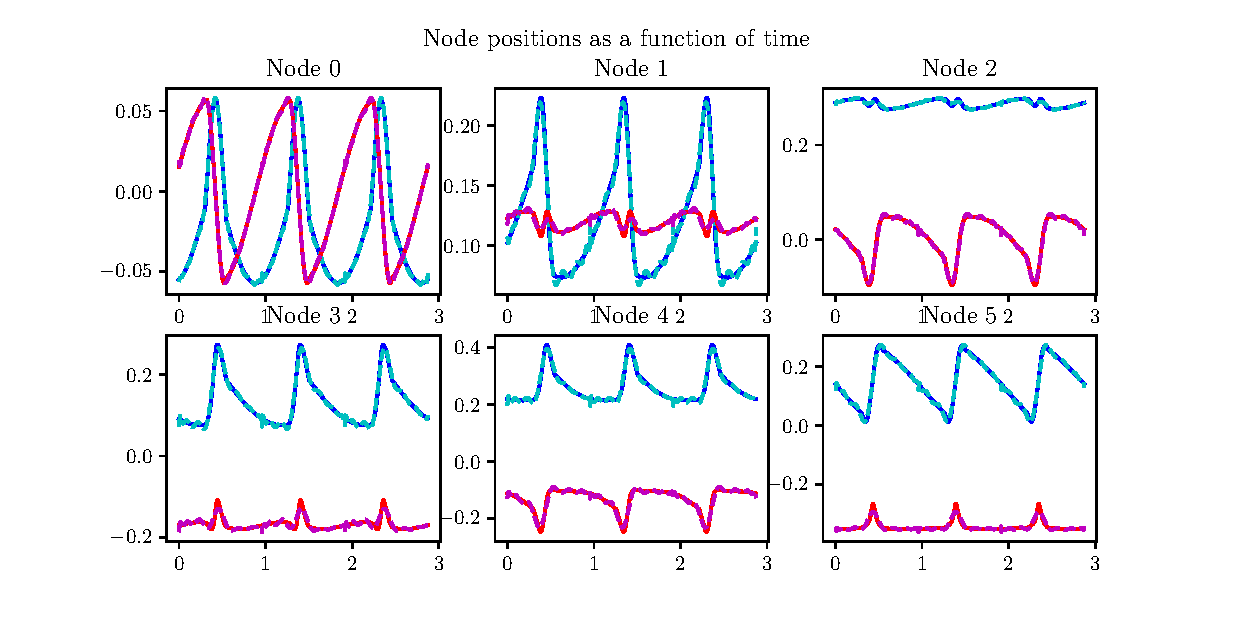
\includegraphics[width=\textwidth]{images/4/4_node-positions-fct-of-time.eps}
    \caption[Comparison between actual node trajectories and approximated trajectories over three leg cycles]{Comparison between actual node trajectories and approximated trajectories over three leg cycles. The original node position in $x$ is given in blue, the polynomial fit is given in cyan, the original node position in $y$ is given in red, and the polynomial fit is given in magenta}
    \label{fig:4_node-positions-fct-of-time}
\end{figure}

\subsubsection{Dynamic Model}

The dynamic model was fully developed using the same set equations as shown for the 3-DoF series-articulated topology. It was found, however, that this approach requires the use of Lagrange multipliers to represent the constraints applied to the leg \cite{nansai_dynamic_2013}. Without these, for a constant motor velocity during the contact and flight phases, the inertial terms are equal to zero. Equally, the external force is mostly lost. Both these significant inaccuracies are captured in Figure \ref{fig:4_jansen-torques}.

\begin{figure}
    \centering
    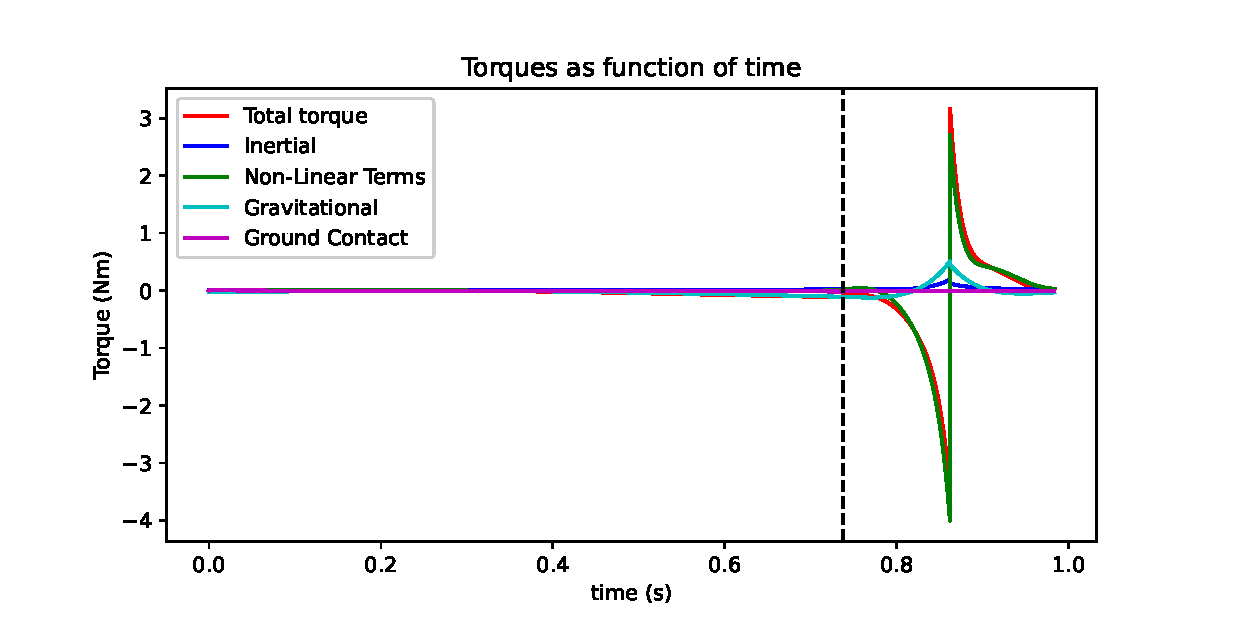
\includegraphics[width=\textwidth]{images/4/4_jansen-torques.eps}
    \caption[Improper Jansen torques found in dynamic model as a function of time over a leg cycle]{Improper Jansen torques found in dynamic model as a function of time over a leg cycle. The black dotted line indicates when the leg shifts from the ground contact phase (leg must carry weight of the robot) to flight phase.}
    \label{fig:4_jansen-torques}
\end{figure}

The leg dynamics were instead developed using Free Body Diagrams to determine the reaction forces at each link, beginning at the foot at Node-5 and working up to the actuator; a sample diagram is given by Figure \ref{fig:4_jansen-free-body-diagram}. The equations for each node are presented from (\ref{eq:jansen_reaction_5}) to (\ref{eq:jansen_reaction_torque}) in the order in which they are solved for; reaction $R_i$ correspond to the internal forces required to achieve the node accelerations $\ddot{x_i}$ and $\ddot{y_i}$. $\tau$ represents the output torque at the actuator, while mass $m_i$ represents the mass of link $i$ as per Figure \ref{fig:4_jansen-mechanism-patnaik}. Node-1 and Node-2 were not analysed directly; instead, links $\ell_2$, $\ell_{9}$ and $ell_{10}$ were treated as a solid body, and the sum of moments, illustrated in Figure \ref{fig:4_jansen_fbd_solid_body}, was solved for $R_1$.

\begin{figure}
    \centering
    \includegraphics[width=0.7\textwidth]{images/4/4_jansen_fbd_example.png}
    \caption{Sample Free-Body Diagram for Node-5}
    \label{fig:4_jansen-free-body-diagram}
\end{figure}

\begin{figure}
    \centering
    \includegraphics[width=0.8\textwidth]{images/4/4_jansen_fbd_solid_body.png}
    \caption{Free-Body Diagram for solid body composed of links $\ell_2$, $\ell_9$ and $\ell_{10}$}
    \label{fig:4_jansen_fbd_solid_body}
\end{figure}

\begin{align}
    R_5 &= \frac{(\frac{m_4+m_5}{2})(\ddot{y_5} + g - \ddot{x_5}\tan\theta_4) - F_e}{\sin\theta_5 - \cos\theta_5\tan\theta_4} \label{eq:jansen_reaction_5}
    \\
    R_4 &= \frac{(\frac{m_4+m_5}{2}) - R_5\cos\theta_5}{\cos\theta_4}
    \\
    R_7 &= \frac{(\frac{m_3+m_7}{2})(\ddot{y_4} + g - \ddot{x_4}\tan\theta_3) + R_4(\sin\theta_4 - \cos\theta_4\tan\theta_3)}{\sin\theta_7 - \cos\theta_7\tan\theta_3}
    \\
    R_3 &= \frac{(\frac{m_3+m_7}{2})\ddot{x_4} - R_7\cos\theta_7 + R_4\cos\theta_4}{\cos\theta_3}
    \\
    R_8 &= \frac{(\frac{m_6+m_8}{2})(\ddot{y_3} + g - \ddot{x_3}\tan\theta_3) + R_5(\sin\theta_5 - \cos\theta_5\tan\theta_6)}{\sin\theta_8 - \cos\theta_8\tan\theta_6} \\
    &\quad +  \frac{R_7(\sin\theta_6-\cos\theta_7\tan\theta_7)}{\sin\theta_8 - \cos\theta_8\tan\theta_6}
    \\
    R_6 &= \frac{(\frac{m_6+m_8}{2})\ddot{x_3} - R_8\cos\theta_8 + R_5\cos\theta_5 + R_7\cos\theta_7}{\cos\theta_6}
    \\
    \alpha &= \frac{\sqrt{\ddot{x}_2^2 + \ddot{y}_2^2} \cos\left(\theta_3 - \left(\frac{\pi}{2}+\theta_{10}\right)\right)}{\ell_{10}}
    \\
    R_1 &= \frac{\left(\frac{m_1+m_2+m_9}{2}\ell_9^2 + \frac{m_2+m_3+m_10}{2}\ell_{10}^2\right)\alpha + R_3 \ell_{10} \left(\cos\theta_3 \sin\theta_{10} + \sin\theta_3 \cos\theta{10} \right)}{\cos\theta_1 \sin\theta_9 + \sin\theta_1 \cos\theta_9}
    \\
	\tau &= \frac{m_0+m_1+m_6}{2} g \ell_0 \cos\theta_0 + R_1 \ell_0 (\sin\theta_1 \cos\theta_0 - \cos\theta_1 \sin\theta_0) \\
	&\quad + R_6 \ell_0 (\sin\theta_6 \cos\theta_0 - \cos\theta_6 \sin\theta_0) \label{eq:jansen_reaction_torque}
\end{align}

For the reaction $R_5$, the external force term $F_e$ represents the mass of the robot which must be held up by the leg, equal to the sum of all link masses and one third the torso mass of the robot, as the torso mass is shared between the three legs participating in the stable stance at any time. $F_e$ is therefore only present in the equation during the stance phase, when the leg is in contact with the ground. The link masses are split between their extremities and link inertias are neglected.

\subsubsection{Singularities}

Previously, a free body diagram was developed for each node, and link reaction equations derived. This methodology resulted in three additional equations.

\begin{align}
    R_2 &= \frac{(m_2+m_{10})\ddot{x_2} - R_{10}\cos\theta_{10} + R_3\cos\theta_3}{\cos\theta_2}
    \\
    R_9 &= \frac{(m_1+m_9)(\ddot{y_1} + g - \ddot{x_1}\tan\theta_1) + R_2(\sin\theta_2 - \cos\theta_2 \tan\theta_1)}{\sin\theta_9 - \cos\theta_9 \tan\theta_1}
    \\
    R_{10} &= \frac{(m_2+m_10)(\ddot{y_2} + g - \ddot{x_2}\tan\theta_2) + R_3(\sin\theta_3 - \cos\theta_3 \tan\theta_2)}{\sin\theta_{10} - \cos\theta_{10} \tan\theta_2} \label{eq:jansen_R10}
\end{align}

Using this method gave the torque graph shown in Figure \ref{fig:5_jansen_torque_invalid}. The massive torque spikes can be traced back to the reaction force $R_{10}$, shown in Figure \ref{fig:5_jansen_R10}.

\begin{figure}[b]
    \centering
    \includegraphics[width=\textwidth]{images/5/5_torque_invalid.png}
    \caption{Torque output of Jansen linkage over a three leg cycles without correcting for singularities}
    \label{fig:5_jansen_torque_invalid}
\end{figure}

\begin{figure}
    \centering
    \includegraphics[width=\textwidth]{images/5/5_R10.png}
    \caption{Reaction $R_{10}$ as a function of time}
    \label{fig:5_jansen_R10}
\end{figure}

These spikes are largely explained by the presence of modelling singularities; positions in which the reaction expressions tend towards infinity due to the presence of an asymptotic function. The force spikes present in Figure \ref{fig:5_jansen_R10} align chronologically with the times during which $R_{10}$'s denominator as defined in (\ref{eq:jansen_R10}) is equal to zero, and thus there is a reaction of infinite amplitude. Since reaction $R_{10}$ is used to determine the reactions $R_1$, $R_2$ and $R_9$, and subsequently the actuator torque $\tau$, these all exhibit the same large spikes, as shown in Figure \ref{fig:5_jansen_reactions_invalid}.

\begin{figure}
    \centering
    \includegraphics[width=\textwidth]{images/5/5_R10_denominator.png}
    \caption[Factors of $R_{10}$ denominator]{Factors of $R_{10}$ denominator. As per (\ref{eq:jansen_R10}), the denominator takes the form $\sin\theta_{10} - \cos\theta_{10}\tan\theta_2$}
    \label{fig:5_jansen_R10_denom}
\end{figure}

\begin{figure}
    \centering
    \includegraphics[width=\textwidth]{images/5/5_reactions_over_time_invalid.png}
    \caption[Reaction forces of Jansen linkage over a three leg cycles without correcting for singularities]{Reaction forces of Jansen linkage over a three leg cycles without correcting for singularities. Reaction $R_{10}$ is not shown, but exhibits a similar form to reactions 1, 2 and 9}
    \label{fig:5_jansen_reactions_invalid}
\end{figure}

It is worth noting that this singularity is not mechanical; one of the singular leg configurations is shown in Figure \ref{fig:5_jansen_singular_configuration_1}. The leg is fully capable of moving in and out of this position. The singularity is thus a consequence of the modelling technique, and not the leg design.

\begin{figure}
    \centering
    \includegraphics[width=0.8\textwidth]{images/5/5_R10_overflow_singular_configuration_1.png}
    \caption[Jansen linkage leg configuration during larger of the two singularities]{Jansen linkage leg configuration during larger of the two singularities. The left red dot represents the actuator, the right one represents the pin, the red link represents link $R_{10}$, for whom the reaction force tends towards infinity, and the blue curve represents the trajectory taken by the foot}
    \label{fig:5_jansen_singular_configuration_1}
\end{figure}

When the Jacobian is used for forward and inverse kinematics, and the dynamic model, techniques such the damped least-squares method or Moore-Penrose Pseudoinverse are used to approximate the appropriate value when such as singularity is found \cite{chiaverini_review_1994}\cite{sciencedirect_moore-penrose_nodate}. Alternatively, treating links $\ell_2$, $\ell_9$ and $\ell_{10}$ as forming a solid body avoids the mathematically singular configurations present in (\ref{eq:jansen_R10}).

\begin{comment}
%%%%%%%%%%%%%%%%%%%%%%%%%%%%%%%%%%%%%%%%%%%%%%%%%%%%%%%%%%%
%  3-DoF series-articulated
%%%%%%%%%%%%%%%%%%%%%%%%%%%%%%%%%%%%%%%%%%%%%%%%%%%%%%%%%%%
\subsection{Underactuated Spatial Mechanism}

Whereas the proportions of other leg topologies are based on existing quadrupeds, the underactuated configuration with three sets of linkages must undergo more careful deliberation, as this design will result in an uncontrolled degree of freedom whose orientation should be placed to maximize performance. Sample configurations are shown in Figure \ref{fig:parallel_concept_top}.

\begin{figure}
    \centering
    \includegraphics[width=0.8\textwidth]{4/4_parallel_top.png}
    \caption{Possible configurations for underactuated spatial leg topology}
    \label{fig:parallel_concept_top}
\end{figure}
\end{comment}